%%%%%%%%%%%%%%%%%%%%%%%%%%%%%%%%%%%%%%%%%
% Multi-Purpose Large Font
% LaTeX Template
%
% This template has been downloaded from:
% http://www.LaTeXTemplates.com
%
% Original author:
% Frits Wenneker (http://www.howtotex.com)
%
% This template can be used in one of two ways:
%
% 1) Content can be added at the end of this file just before the \end{document}
% to use this title page as the starting point for your document.
%
% 2) Alternatively, if you already have a document which you wish to add this
% title page to, copy everything between the \begin{document} and
% \end{document} and paste it where you would like the title page in your
% document. You will then need to insert the packages and document 
% configurations into your document carefully making sure you are not loading
% the same package twice and that there are no clashes.
%
%%%%%%%%%%%%%%%%%%%%%%%%%%%%%%%%%%%%%%%%%

%----------------------------------------------------------------------------------------
%	PACKAGES AND OTHER DOCUMENT CONFIGURATIONS
%----------------------------------------------------------------------------------------

\documentclass[11pt]{article}

\usepackage[a4paper,pdftex]{geometry}	% Use A4 paper margins
\usepackage[english]{babel}
\usepackage{xcolor} % Required for specifying custom colors
\usepackage{fix-cm} % Allows increasing the font size of specific fonts beyond LaTeX default specifications
\usepackage{graphicx}
\usepackage{amsmath}
\usepackage{float}

\setlength{\oddsidemargin}{0mm} % Adjust margins to center the colored title box
\setlength{\evensidemargin}{0mm} % Margins on even pages - only necessary if adding more content to this template

\newcommand{\HRule}[1]{\hfill \rule{0.2\linewidth}{#1}} % Horizontal rule at the bottom of the page, adjust width here

\definecolor{grey}{rgb}{0.9,0.9,0.9} % Color of the box surrounding the title - these values can be changed to give the box a different color	

\begin{document}

\thispagestyle{empty} % Remove page numbering on this page

%----------------------------------------------------------------------------------------
%	TITLE SECTION
%----------------------------------------------------------------------------------------

\colorbox{grey}{
	\parbox[t]{1.0\linewidth}{
		\centering \fontsize{50pt}{80pt}\selectfont % The first argument for fontsize is the font size of the text and the second is the line spacing - you may need to play with these for your particular title
		\vspace*{0.7cm} % Space between the start of the title and the top of the grey box

		\hfill Report-2\par
		
		\vspace*{0.7cm} % Space between the end of the title and the bottom of the grey box
	}
}

%----------------------------------------------------------------------------------------

\vfill % Space between the title box and author information

%----------------------------------------------------------------------------------------
%	AUTHOR NAME AND INFORMATION SECTION
%----------------------------------------------------------------------------------------

{\centering \large 
\hfill Goutam Y G \\
\hfill Saarland University \\

\HRule{1pt}} % Horizontal line, thickness changed here

%----------------------------------------------------------------------------------------

\clearpage % Whitespace to the end of the page

%%%%%%%%%%%%%%%%%%%%%%%%%%%%%%%%%%%%%%%%%%%%%%%%%%%%%%%%%%%%%%%%%%%%%%%%%%%%%%%%%%%%%%%%%

\newpage

\textbf{Motivation:}
\\\\
While training the neural networks, back-propagation is used to update the network weights. This is equivalent to the gradient descent method, where one takes a step in the direction of descent on the error surface. Low curvature regions on the error surface of the network result in slow progress and sometimes termination of the algorithm. Newton’s method handles cases with low curvature and takes larger steps (step size inversely to
the curvature). It reaches the global minimum if the function is quadratic. If the function is non-quadratic, then it may converge to a saddle point, relative maxima or it may diverge.(See the introduction part of \cite{oke})
\\\\
A modified version of Newton’s method, called \textbf{Saddle-Free Newton(SFN)} was proposed in a research paper by Dauphin et al.\cite{dauphin} SFN replaces the hessian matrix by a semi-definite matrix which is obtained by replacing the eigenvalues of the Hessian by their absolute values. Empirical results using 2D functions show that SFN escapes saddle points.
\\\\
For a function $f(x)$, Newton’s method does a quadratic approximation at the point x and minimizes it. By using the matrix defined in SFN, we use a positive semi-definite matrix derived from the Hessian and approximate the surface by a quadratic function. If the approximation is bad, then the resultant direction might be arbitrary. We suspect that there are cases in which SFN updates result in ascent/arbitrary directions which are not desirable.
\\\\
Also, computation of Hessian is a very expensive operation. It is interesting to see if some of the less expensive first order methods like momentum, rmsprop, ADAM etc. can escape saddle points and handle low curvature regions.
\\\\
\textbf{Experiment}:
\\\\First we analyze the behavior of gradient descent, Newton and SFN on various 2D functions. We note down different factors like - possible challenges (low curvature, multiple stationary points, saddle points etc), initialization, number of iterations, reason for termination etc. for each method. Also, we visualize the path taken by all the algorithms on the function surface.
%%%%%%%%%%%%%%%%%%%%%%%%%%%%%%%%%%%%%%%%%%%%%%%%%%%%%%%%%%%%%%%%%%%%%%%%%%%%%%%%%%%%%%%%%

\newpage

Function: $3x^2-y^2$
\\\\
Challenges: It has a saddle point at (0, 0)
\\\\
Initialization Point is (1.3, −0.3), which is close to the saddle point. $f$(1.3,-0.3) = 4.98.
\\\\
\textbf{Gradient Descent}: Learning rate $\alpha$ = 0.01
\\Termination Point:(−0.0046, −4.0326) and $f$(-0.0046,-4.0326) = -16.2617.
\\Reason for termination: Out of range (After escaping the saddle point)
\\Number of steps taken: 132
\\Computational time: 60 ms
\\\\
\textbf{Newton’s Method}: 
\\Termination Point: (−0.0050, −0.0050) and $f$(-0.0050,-0.0050) = $5 ∗ 10^{-5}$
\\Reason for termination: Convergence at the saddle point(L2 norm of difference vector between two successive points is less than $10^{-5}$ )
\\Number of steps taken: 2
\\Computational time: 20 ms
\\\\
\textbf{SFN}: 
\\Termination Point: (−0.0005, −4.7925) and $f$(-0.0005,-4.7925) = -22.9681
\\Reason for termination: Out of range (After escaping the saddle point)
\\Number of steps taken: 4
\\Computational time: 12 ms

\begin{figure}[H]
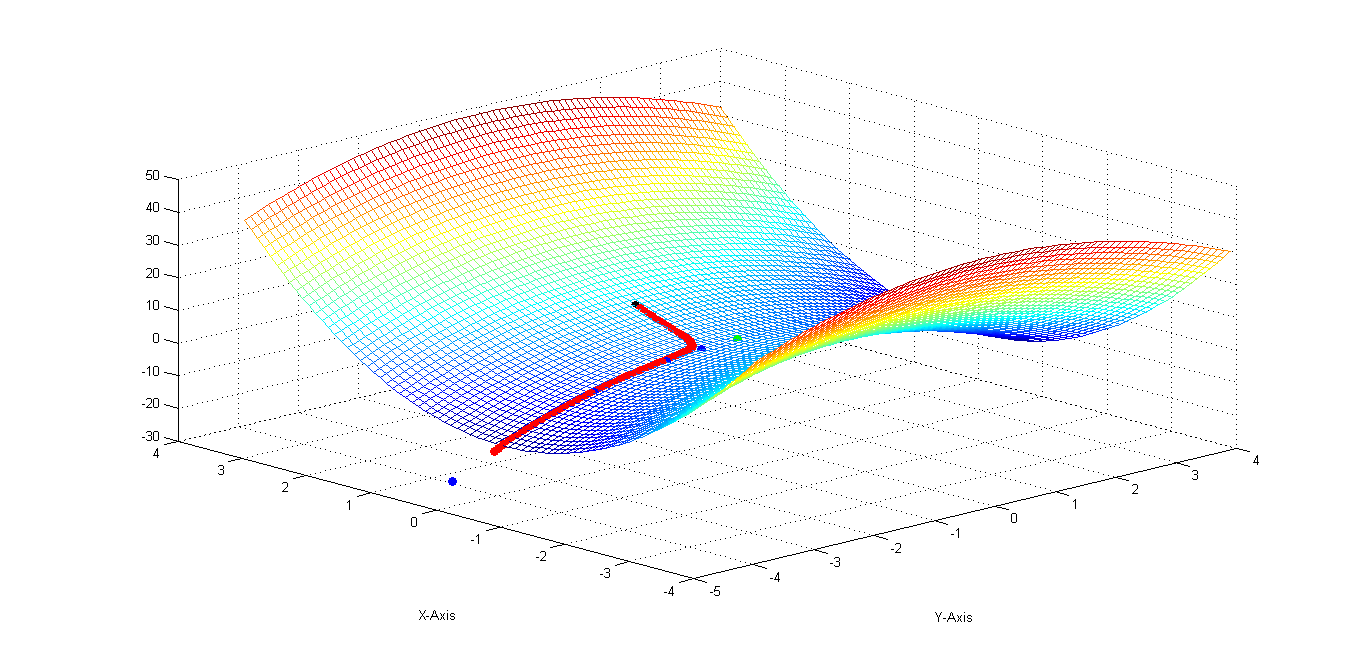
\includegraphics[scale = 0.45]{1.png}
\caption{Initialization-Black, Gradient Descent-Red, Newton-Green, SFN-Blue}
\end{figure}

%%%%%%%%%%%%%%%%%%%%%%%%%%%%%%%%%%%%%%%%%%%%%%%%%%%%%%%%%%%%%%%%%%%%%%%%%%%%%%%%%%%%%%%%%

\newpage

Function: $x^3-3xy^2$
\\\\
Challenges: It has a saddle point at (0, 0)
\\\\
Initialization Point is (3.5, 0.5) and $f$(3.5,0.5) = 40.25
\\\\
\textbf{Gradient Descent}: Learning rate $\alpha$ = 0.01
\\Termination Point:(2.5664, 4.1059) and $f$(2.5664,4.1059) = -112.8945
\\Reason for termination: Out of range (After escaping the saddle point)
\\Number of steps taken: 16
\\Computational time: 20 ms
\\\\
\textbf{Newton’s Method}:
\\Termination Point: (0, 0) and $f$(0,0) = 0.
\\Reason for termination: Convergence at the saddle point(L2 norm of difference vector between two successive points is less than $10^{-5}$).
\\Number of steps taken: 25
\\Computational time: 27 ms
\\\\
\textbf{SFN}: 
\\Termination Point: (2.5185, 4.3629) and $f$(2.5185,4.3629) = -127.845
\\Reason for termination: Out of range (After escaping the saddle point)
\\Number of steps taken: 4
\\Computational time: 17 ms

\begin{figure}[H]
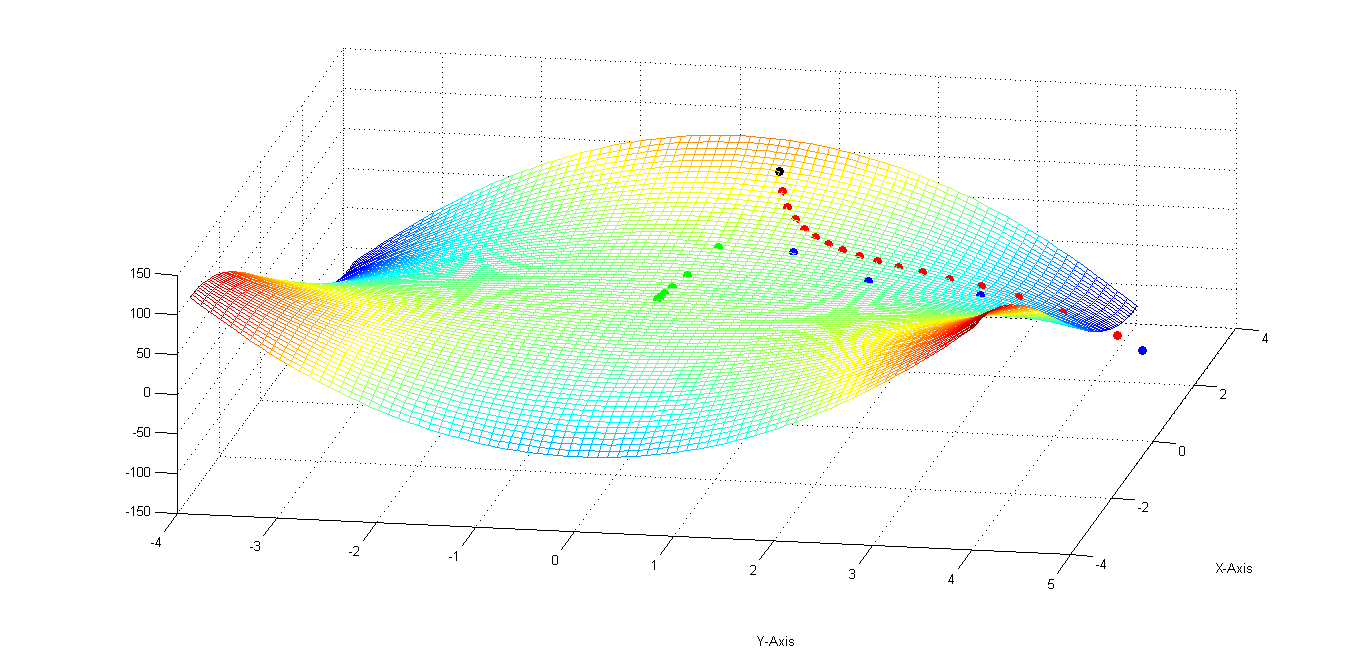
\includegraphics[scale = 0.45]{2.png}
\caption{Initialization-Black, Gradient Descent-Red, Newton-Green, SFN-Blue}
\end{figure}

%%%%%%%%%%%%%%%%%%%%%%%%%%%%%%%%%%%%%%%%%%%%%%%%%%%%%%%%%%%%%%%%%%%%%%%%%%%%%%%%%%%%%%%%%

\newpage

Function: $x^3-y^3-3x+3y$
\\\\
Challenges: The function has 4 stationary points: (1,1),(1,-1),(-1,1) and (-1,-1). (1,-1) is a local minimum, (-1,1) is a local maximum, (1,1) and (-1,-1) are saddle points.
\\\\
The Hessian at any point(x,y) is of the form [6x 0;0 -6y]. For any point with values of x and y close to zero, the Hessian has small eigenvalues. It will be interesting to see the behavior of Newton, SFN which rely on the Hessian.
\\\\
Initialization Point is (0, 0) and $f$(0,0) = 0
\\\\
\textbf{Gradient Descent}: 
\\Learning rate $\alpha$ = 0.01
\\Termination Point:(1, −1) which is a local minimum and $f$(1,-1) = -4.
\\Reason for termination: Convergence at the local minimum(L2 norm of difference vector between two successive points is less than $10^{-5}$).
\\Number of steps taken: 160
\\Computational time: 21 ms
\\\\
\textbf{Newton’s Method}:
\\ Termination Point: (500, 500) and $f$(500,500) = 0.
\\Reason for termination: Out of range (Hessian entries were of the order $10^{-3}$ which resulted in a very large step from the current location)
\\Number of steps taken: 1
\\Computational time: 7 ms
\\\\
\textbf{Note}: By ignoring the out of range condition for termination, it is observed that New-
ton’s method converges to the saddle point (1, 1) after 14 iterations.
\\\\
\textbf{SFN}: 
\\Termination Point: (500, −500) and $f$(500,-500) = $2.5*10^8$
\\Reason for termination: Out of range (Hessian entries were of the order $10^{-3}$ which resulted in a very large step from the current location)
\\Number of steps taken: 1
\\Computational time: 1 ms
\\\\
\textbf{Note}: By ignoring the out of range condition for termination, it is observed that SFN converges to the local minimum (1, −1) after 14 iterations.

\newpage

\begin{figure}[H]
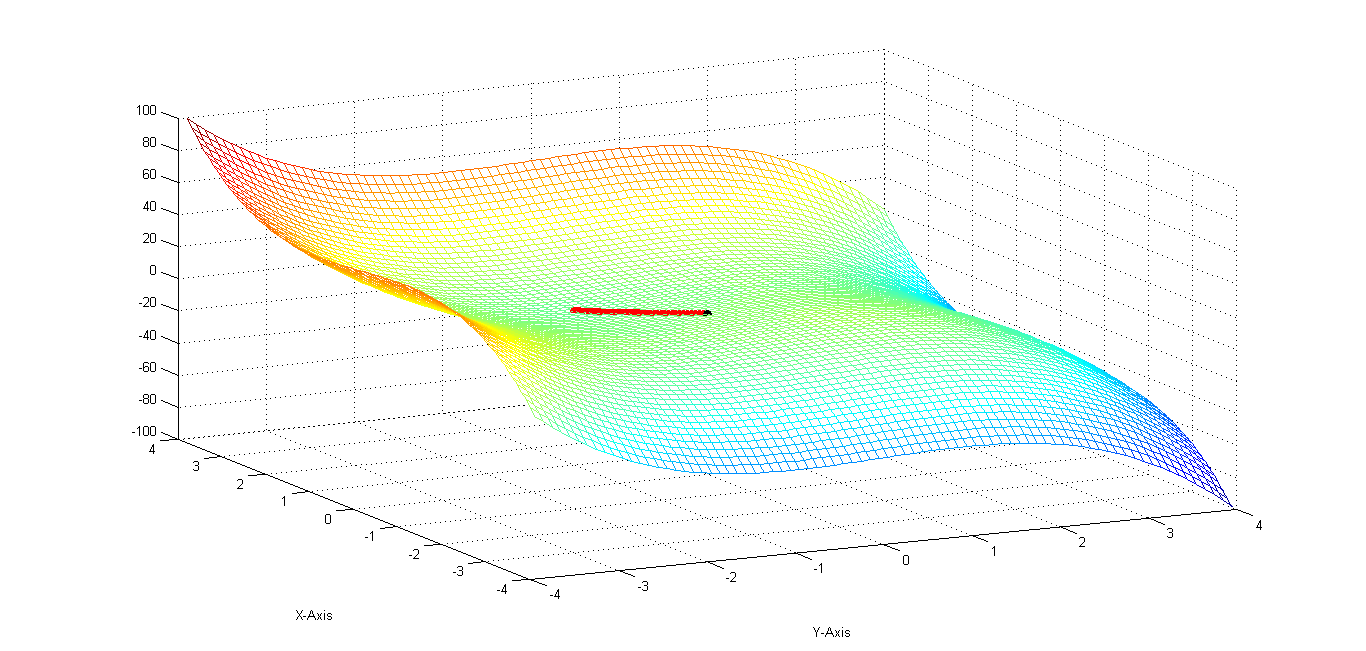
\includegraphics[scale = 0.5]{3.png}
\caption{Initialization-Black, Gradient Descent-Red}
\end{figure}

* Second Initialization Point: (0,0.5) and $f$(0,0.5) = 1.3750
\\\\
\textbf{Gradient Descent}: 
\\Learning rate $\alpha$= 0.01
\\Termination Point:(1,-1) which is a local minimum and $f$(1,-1) = -4
\\Reason for termination: Convergence at the local minimum(L2 norm of difference vector between two successive points is less than $10^{-5}$ ).
\\Number of steps taken: 173
\\Computational time: 25 ms
\\\\
\textbf{Newton’s Method}: 
\\Termination Point: (500, 1.248) and $f$(500,1.248) = $1.25*10^8$
\\Reason for termination: Out of range (Eigenvalues of the Hessian were 0,-3 which resulted in a very large step along x-axis)
Number of steps taken: 1
Computational time: 7 ms
\\\\
\textbf{SFN}: 
\\ Termination Point: (500,-0.2480) and f(500,-0.2480) = $1.25*10^8$
\\ Reason for termination: Out of range (Eigenvalues of the modified Hessian were 0,3 which resulted in a very large step along x-axis)
\\ Number of steps taken: 1
\\ Computational time: 2 ms

%%%%%%%%%%%%%%%%%%%%%%%%%%%%%%%%%%%%%%%%%%%%%%%%%%%%%%%%%%%%%%%%%%%%%%%%%%%%%%%%%%%%%%%%%

\newpage

Function: $e^{-(x^2+y^2)}sin(x)sin(y)$

Challenges: $\dfrac{\partial f}{\partial x}$  = $ sin(y)[cos(x)*e^{-(x^2+y^2)} - 2x*sin(x)*e^{-(x^2+y^2)}]$
\\ and $\dfrac{\partial f}{\partial y} = sin(x)[cos(y)*e^{-(x^2+y^2)}-2y*sin(y)*e^{-(x^2+y^2)}]$ are the partial derivatives.
\\\\
The function has a multiple critical points, which can be observed from the equations
above. It has a saddle point at (0,0).(Observed from the plot)
\\\\To find the global maximum/minimum, we need to solve the following equations analytically.
$tan(x) = \dfrac{1}{2x}$ and $tan(y) = \dfrac{1}{2y}$

\begin{figure}[h]
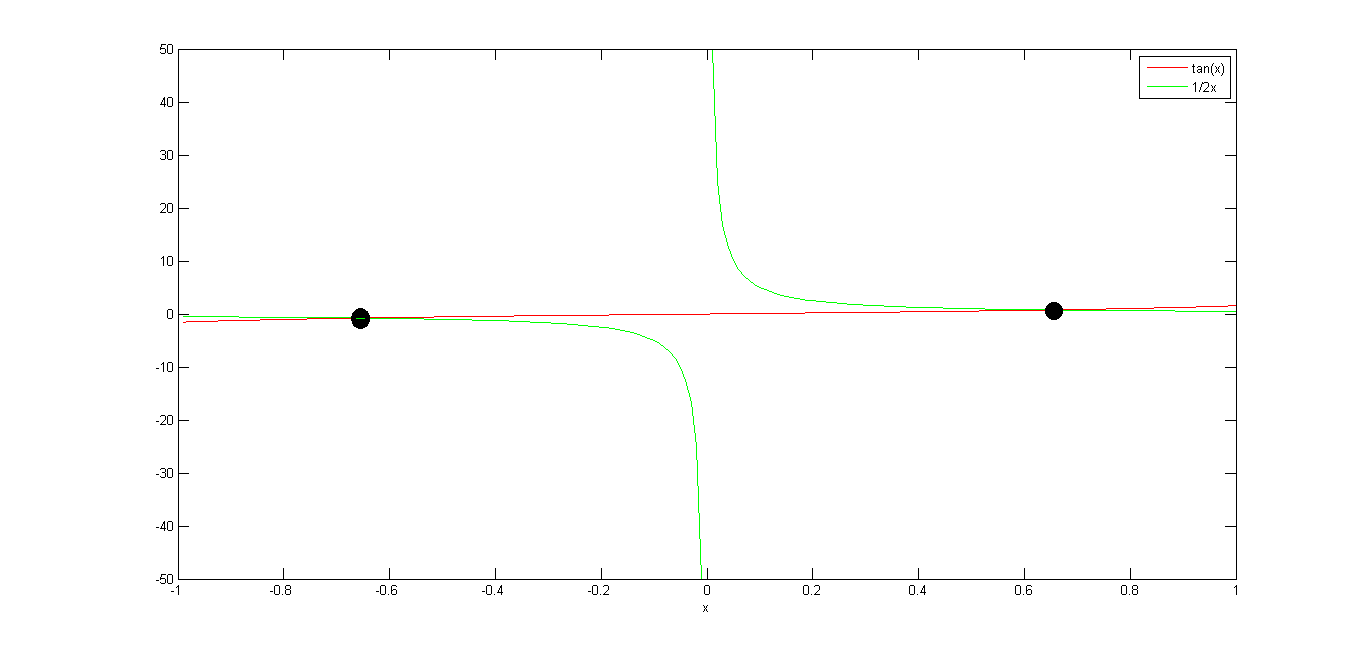
\includegraphics[scale = 0.5]{40.png}
\caption{Plot of $tan(x)$ and $\dfrac{1}{2x}$}
\end{figure}

From the figure above, two functions intersect at around x=0.65 and x=-0.65 in the
interval (-1,1). There are two global maximum at (0.65,0.65),(-0.65,-0.65) and two global
minimum at (-0.65,0.65),(0.65,-0.65).
\\
\\Initialization Point: (0.4,0.2) and f(0.4,0.2) = 0.0633
\\\\
\textbf{Gradient Descent}:
\\Learning rate $\alpha$ = 0.1
\\Termination Point:(0.6537, −0.6537) which is a global minimum and $f$(0.6537,-0.6537)= -0.1573
\\Reason for termination: Convergence at a global minimum(L2 norm of difference vector between two successive points is less than $10^{-5}$).
\\Number of steps taken: 122
\\Computational time: 24 ms
\\\\
\textbf{Newton’s Method}: 
\\Termination Point:(-4.8318,-4.5676) and $f$(-4.8318,-4.5676) = 0
\\Reason for termination: Out of range (Eigenvalues of the Hessian were 0.03,-0.86 which resulted in a very large step)
\\Number of steps taken: 1
\\Computational time: 7 ms
\\\\
\textbf{SFN}: 
\\Termination Point: (-4.6080,-4.8021) and $f$(-4.6080,-4.8021) = 0
\\Reason for termination: Out of range (Eigenvalues of the modified Hessian were 0.03,0.86 which resulted in a very large step)
\\Number of steps taken: 1
\\Computational time: 18 ms

\begin{figure}[H]
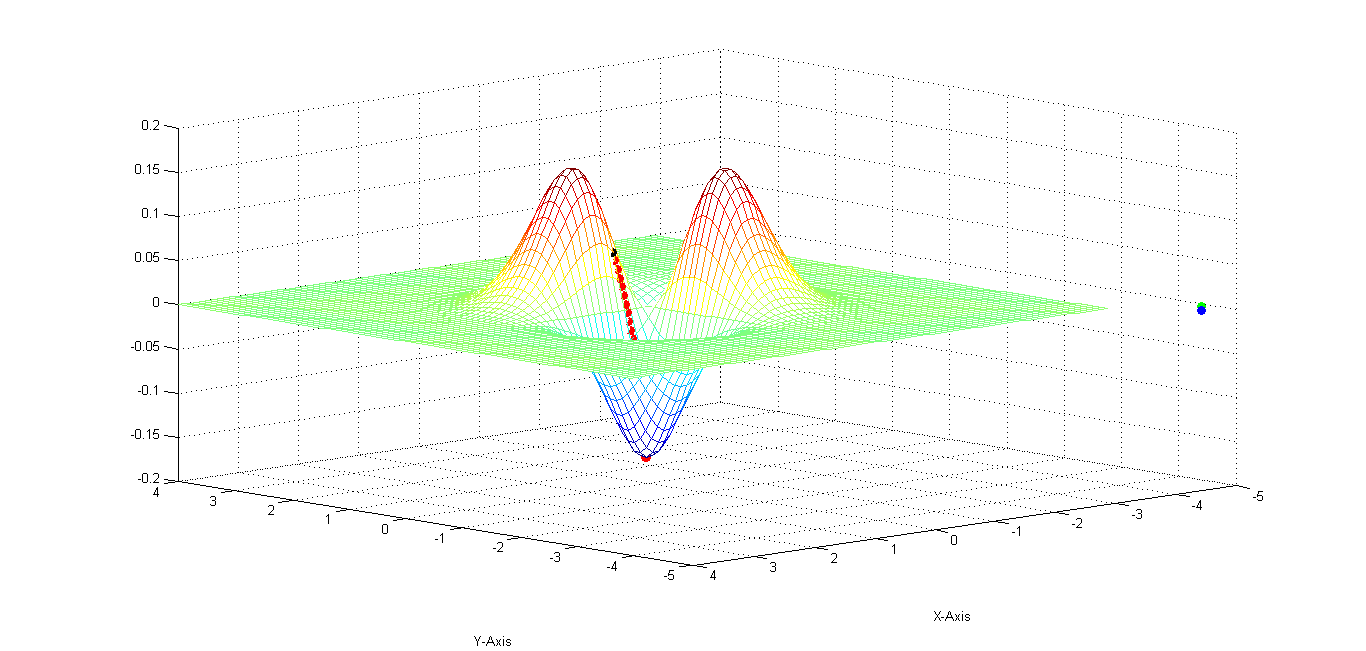
\includegraphics[scale = 0.5]{4.png}
\caption{Initialization-Black, Gradient Descent-Red, Newton-Green, SFN-Blue}
\end{figure}

%%%%%%%%%%%%%%%%%%%%%%%%%%%%%%%%%%%%%%%%%%%%%%%%%%%%%%%%%%%%%%%%%%%%%%%%%%%%%%%%%%%%%%%%%

\newpage

Function: $cos(x)*sin(y)$
\\Challenges: $\dfrac{\partial f}{\partial x} = -sin(x)sin(y)$ and $\dfrac{\partial f}{\partial y} = cos(x)cos(y)$
\\The function has multiple critical points. In the range of (-2.5,2.5), the function has one global maximum at $(0,\dfrac{\pi}{2})$, one global minimum at $(0,\dfrac{-\pi}{2})$ and two saddle points at $(\dfrac{\pi}{2},0)$,$(-\dfrac{\pi}{2},0)$
\\\\For values of x \textbf{and} y close to 0, the determinant of the Hessian tends to 0.\textbf{(ill-conditioned)}
\\\\Initialization Point is (0.1,1.5) and $f$(0.1,1.5) = 0.9925
\\\\
\textbf{Gradient Descent}: 
\\Learning rate α = 0.1
\\Termination Point:$(\pi,\dfrac{\pi}{2})$ which is a global minimum and $f(\pi, \dfrac{\pi}{2})$ = -1
\\Reason for termination: Convergence at a global minimum(L2 norm of difference vector between two successive points is less than $10^{-5}$).
\\Number of steps taken: 136
\\Computational time: 18 ms
\\\\
\textbf{Newton’s Method}: 
\\Termination Point:$(0, \dfrac{\pi}{2})$ and $f(0, \dfrac{\pi}{2})$ = 1
\\Reason for termination: Convergence at a global maximum(L2 norm of difference vector between two successive points is less than $10^{-5}$).
\\Number of steps taken: 3
\\Computational time: 7 ms
\\\\
\textbf{SFN}: 
\\Termination Point: (19.8,-17.8) and $f$(19.8,-17.8) = 0.45
\\Reason for termination: Out of range (At the fourth iteration, the SFN reaches the point (0.8930,0.9195) and the modified Hessian is ill-conditioned and has the eigenvalues 0.02,0.97. It resulted in the algorithm to take a large jump)
\\Number of steps taken: 4
\\Computational time: 20 ms

\begin{figure}[H]
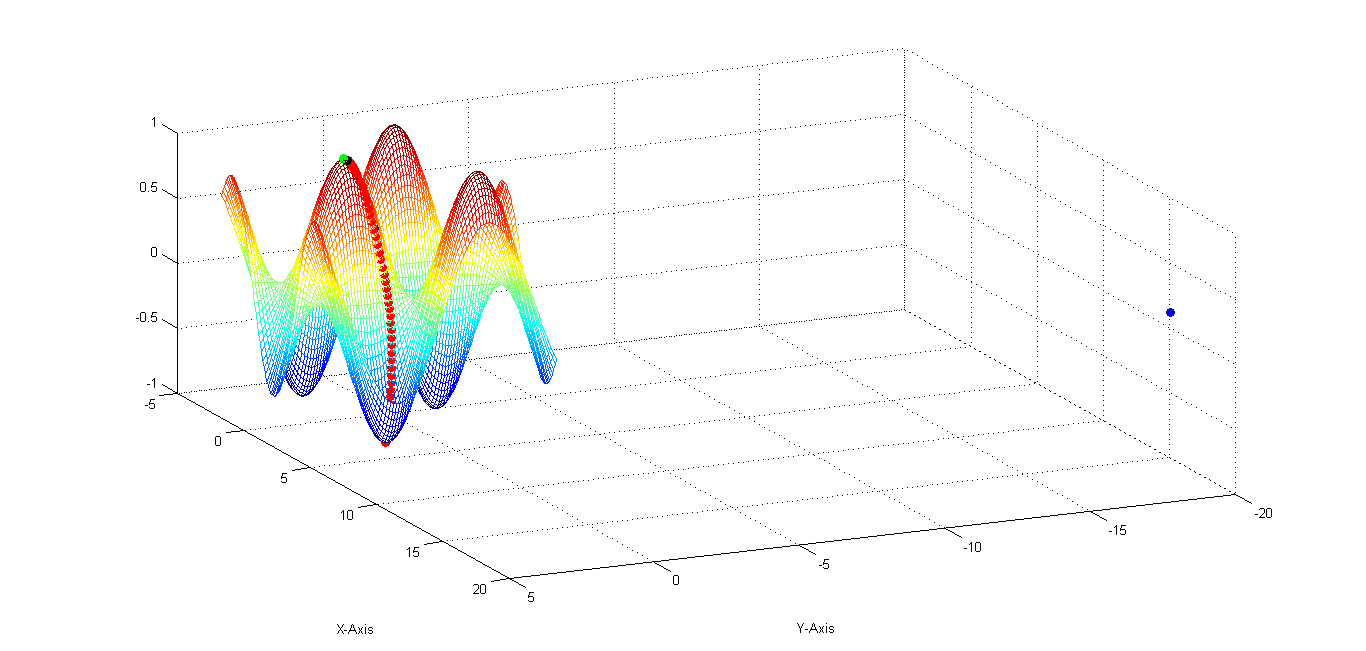
\includegraphics[scale = 0.51]{51.png}
\caption{Initialization-Black, Gradient Descent-Red, Newton-Green, SFN-Blue}
\end{figure}

\begin{figure}[H]
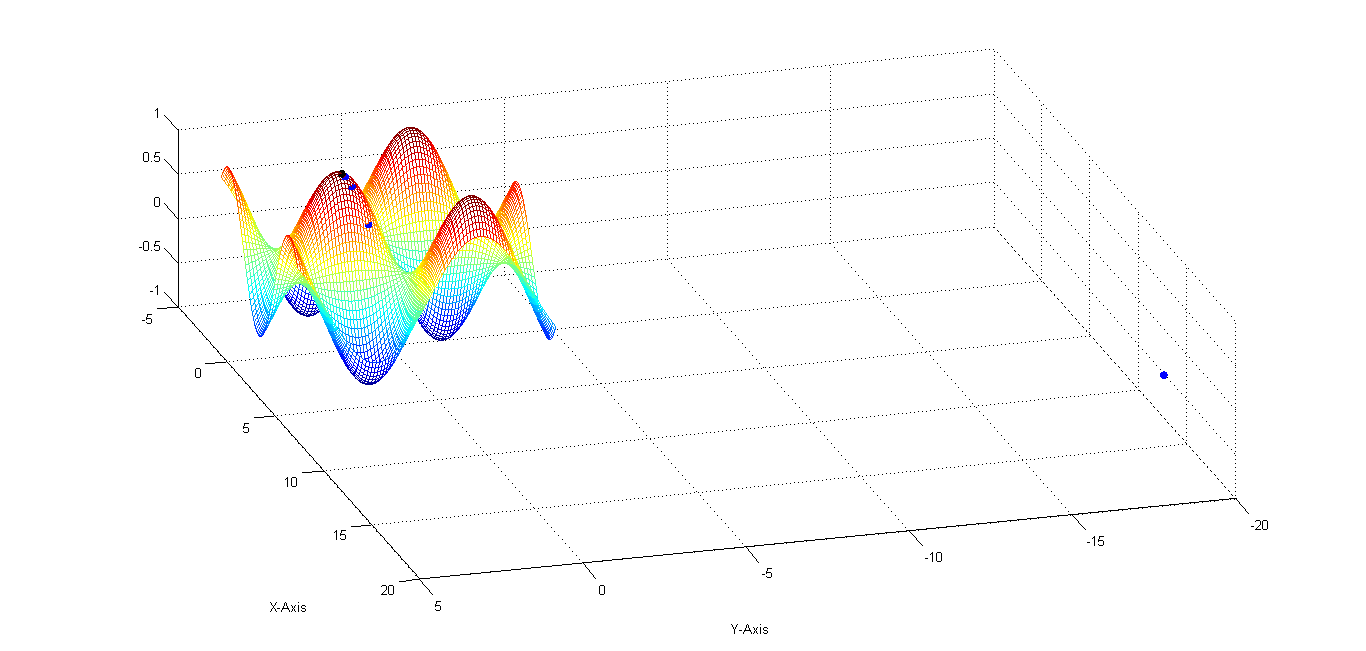
\includegraphics[scale = 0.51]{52.png}
\caption{Path taken by SFN shown separately}
\end{figure}

* Second Initialization at (0,0) and $f$(0,0) = 0
\\\\
\textbf{Gradient Descent}: 
\\Learning rate $\alpha$ = 0.1
\\Termination Point:$(0, -\dfrac{\pi}{2})$ which is a global minimum and $f(0,-\dfrac{\pi}{2})$ = -1
\\Reason for termination: Convergence at a global minimum(L2 norm of difference vector between two successive points is less than $10^{-5}$).
\\Number of steps taken: 96
\\Computational time: 15 ms

\begin{figure}[H]
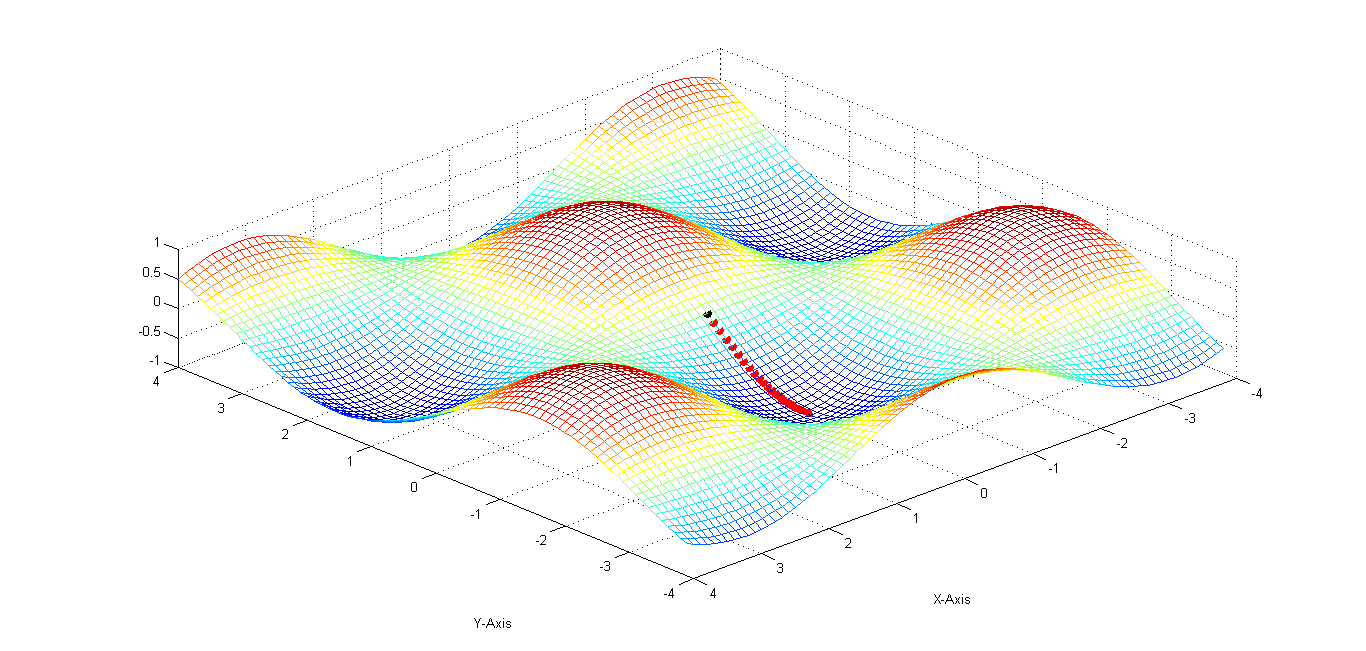
\includegraphics[scale = 0.45]{53.png}
\caption{Path taken by Gradient Descent for (0,0) Initialization}
\end{figure}

\textbf{Newton’s Method}: 
\\Termination Point:(0,2000) and $f$(0,2000) = 0
\\Reason for termination: Out of range(Eigenvalues of the Hessian at (0,0) were $\approx$ 0,0. This resulted in the algorithm take a large jump)
\\Number of steps taken: 1
\\Computational time: 7 ms
\\\\
\textbf{SFN}: 
\\Termination Point: (1414.2,-1414.2) and $f$(1414.2,-1414.2) = -0.4191
\\Reason for termination: Out of range(Eigenvalues of the Hessian at (0,0) were $\approx$ 0,0. This resulted in the algorithm take a large jump)
\\Number of steps taken: 1
\\Computational time: 2 ms

\begin{figure}[H]
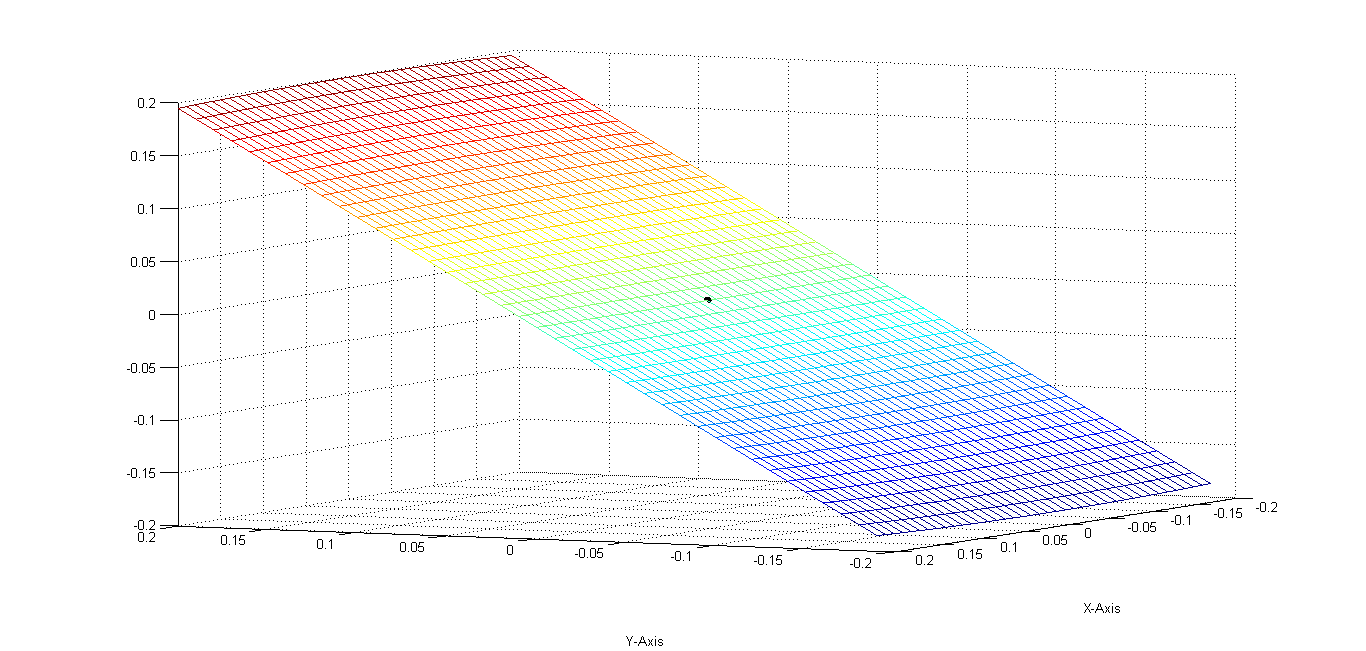
\includegraphics[scale = 0.45]{54.png}
\caption{Newton, SFN behavior near (0,0) explained}
\end{figure}

Above is the plot of the function $cos(x)sin(y)$ in the range (-0.2,0.2) for $x$ and $y$. It can be seen that the function is almost linear and second order derivatives vanish to zero in this case.

%%%%%%%%%%%%%%%%%%%%%%%%%%%%%%%%%%%%%%%%%%%%%%%%%%%%%%%%%%%%%%%%%%%%%%%%%%%%%%%%%%%%%%%%%

\newpage

Function: $x^3 + y^3-3xy$
\\\\Challenges: The function has two critical points, i.e.(0,0) which is a saddle point and (1,1) which is a local minimum.
\\\\The Hessian at any point (x,y) is of the form [2x -1;-1 2y] which can be ill-conditioned for many values of (x,y). It will affect the performance of Newton and SFN.
\\\\
Initialization Point is: (0.4,-0.3) and f(0.4,-0.3) = 0.3970.
\\\\
\textbf{Gradient Descent}: 
\\Learning rate $\alpha$ = 0.01
\\Termination Point:(1,1) which is a local minimum and $f$(1,1) = -1
\\Reason for termination: Convergence at a local minimum(L2 norm of difference vector between two successive points is less than $10^{-5}$).
\\Number of steps taken: 431
\\Computational time: 56 ms
\\\\
\textbf{Newton’s Method}: 
\\Termination Point:(0,0) and $f$(0,0) = 0
\\Reason for termination: Convergence at the saddle point(L2 norm of difference vector between two successive points is less than $10^{-5}$)
\\Number of steps taken: 5
\\Computational time: 9 ms
\\\\
\textbf{SFN}: 
\\Termination Point: (-2.4609,-2.4609) and $f$(-2.4609,-2.4609) = -47.9753
\\Reason for termination: Out of range(After escaping the saddle point, moving towards the global minimum)
\\Number of steps taken: 12
\\Computational time: 5 ms

\begin{figure}[H]
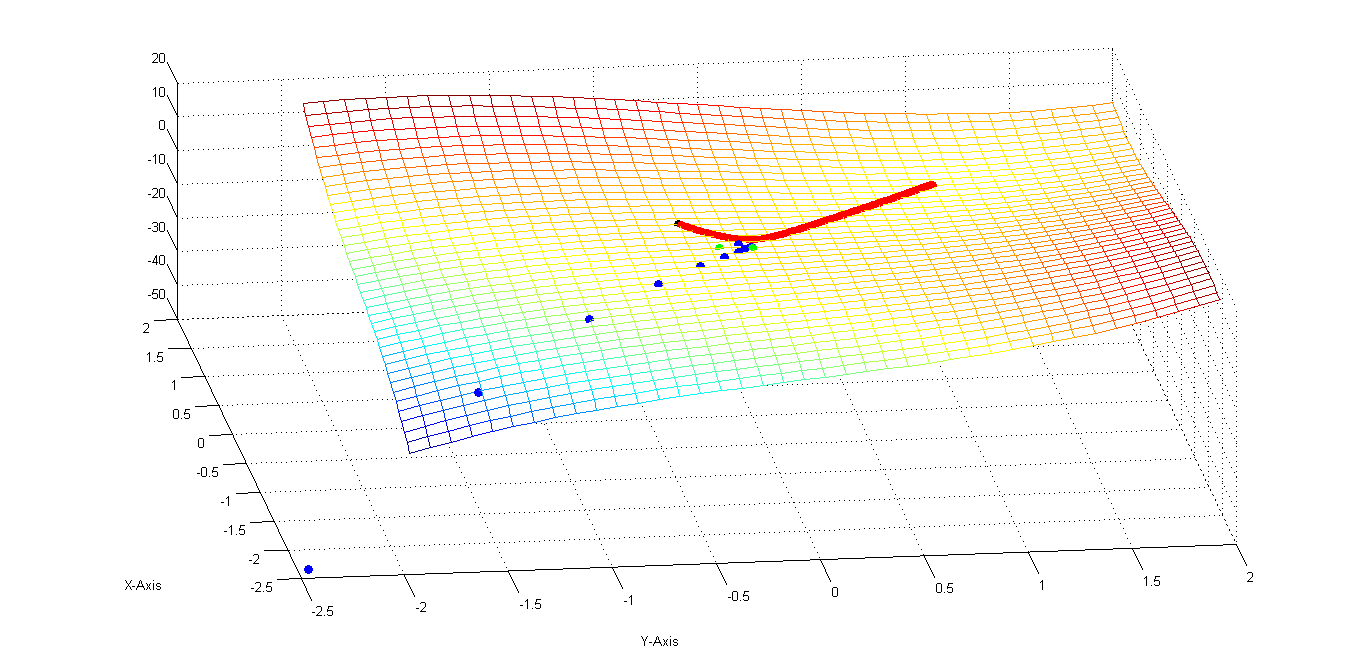
\includegraphics[scale = 0.45]{61.png}
\caption{Initialization-Black, Gradient Descent-Red, Newton-Green, SFN-Blue}
\end{figure}

* Second Initialization Point is: (0.5,0.5) and $f$(0.5,0.5) = -0.5
\\\\
\textbf{Gradient Descent}: 
\\Learning rate $\alpha$ = 0.01
\\Termination Point:(1,1) which is a local minimum and $f$(1,1) = -1
\\Reason for termination: Convergence at a local minimum(L2 norm of difference vector between two successive points is less than $10^{-5}$).
\\Number of steps taken: 277
\\Computational time: 41 ms
\\\\
\textbf{Newton’s Method}: 
\\Termination Point:(125.25,125.25) and $f$(125.25,125.25) = $3.88*10^6$
\\Reason for termination: Out of range(Eigenvalues of the Hessian at (0.5,0.5) were 0,6. This resulted in the algorithm take a large jump)
\\Number of steps taken: 1
\\Computational time: 14 ms
\\\\
\textbf{SFN}: 
\\Termination Point:(125.25,125.25) and f(125.25,125.25) = $3.88*10^6$
\\Reason for termination: Out of range(Eigenvalues of the Hessian at (0.5,0.5) were 0,6. This resulted in the algorithm take a large jump)
\\Number of steps taken: 1
\\Computational time: 2 ms

\begin{figure}[H]
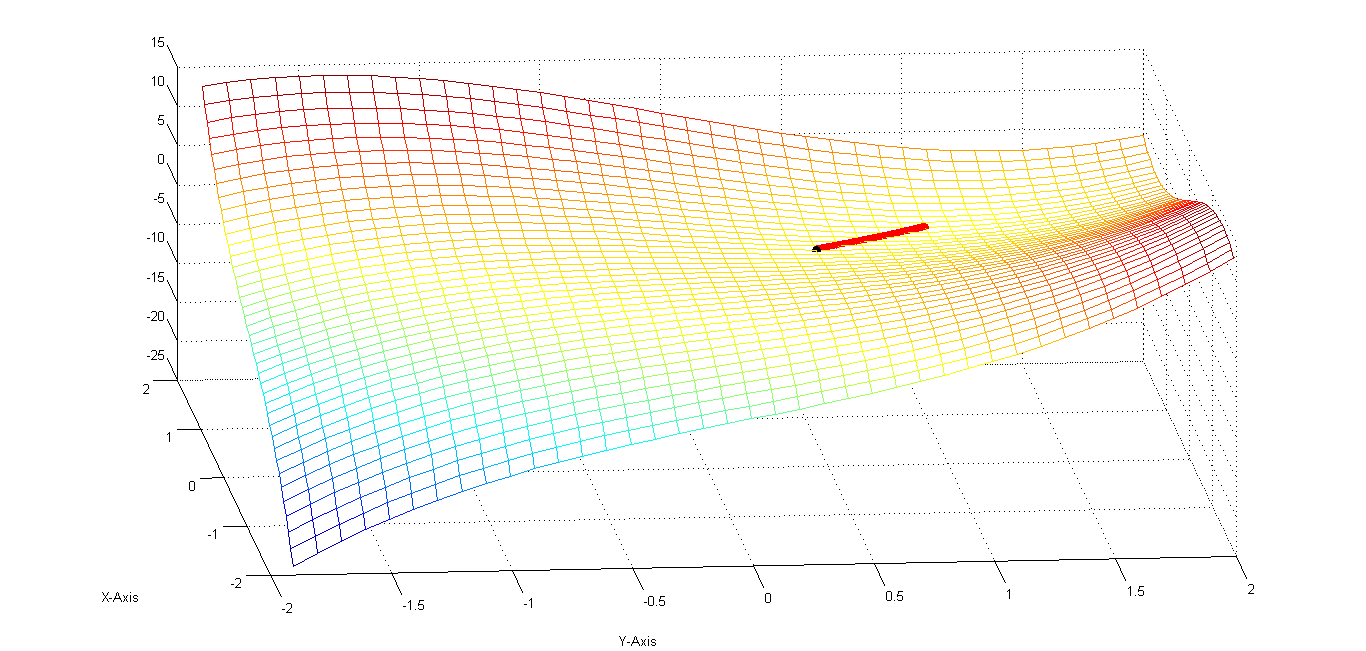
\includegraphics[scale = 0.40]{62.png}
\caption{Gradient Descent for initialization at (0.5,0.5)}
\end{figure}

%%%%%%%%%%%%%%%%%%%%%%%%%%%%%%%%%%%%%%%%%%%%%%%%%%%%%%%%%%%%%%%%%%%%%%%%%%%%%%%%%%%%%%%%%

\textbf{Conclusion}:
\\\\We observe that, SFN works well and escapes saddle points and move towards a minimum faster than gradient descent. But there are cases when Hessian is ill-conditioned(eventhough it is positive definite) and results moving in arbitrary directions. During the experiments, we have shown more of such cases by choosing initialization points/regions where Hessian is ill-conditioned. Probability of SFN algorithm entering such regions might be small in 2D, but it could be a common phenomenon in higher dimensions. (For $10^6*10^6$ Hessian, an eigenvalue being close to/equal to zero is very likely) 
\\\\This raises questions like - (1)Does pre-conditioning the Hessian can solve this problem? (2)Is SFN worth of the computational time we spend to compute the Hessian? (3)Can we explore other first-order methods with adaptive learning rates which are computationally less expensive and escape saddle points?
\\\\Unfortunately we can not make any comment on the computational time aspect, since we are working in 2D.

%%%%%%%%%%%%%%%%%%%%%%%%%%%%%%%%%%%%%%%%%%%%%%%%%%%%%%%%%%%%%%%%%%%%%%%%%%%%%%%%%%%%%%%%%

\begin{thebibliography}{9}

\bibitem{oke}
  M.O. Oke, A Second Order Method for Minimizing Unconstrained Optimization Prob-
lems

\bibitem{dauphin}
Dauphin et al., Identifying and attacking the saddle point problem in high-
dimensional non-convex optimization

\end{thebibliography}


\end{document}